% Poster 2.0 (Mike Morrison "betterposter") style poster.
% Uses Rafael Bailo's betterposter.cls (in this directory).
%
% Build:
%   cd poster && pdflatex poster.tex
%
% A0 landscape by default (1189mm x 841mm). For test prints, use:
%   \documentclass[a1paper]{betterposter}  or  [a2paper]

\documentclass{betterposter}

% Override main-column accent colour to a deep blue more legible than imperial.
\renewcommand{\maincolumnbackgroundcolor}{theory}    % indigo-blue from class
% Other options: empirical (green), methods (red), intervention (yellow)

\usepackage[colorlinks=true,
            urlcolor=blue!60!black,
            citecolor=blue!60!black,
            linkcolor=blue!60!black]{hyperref}

\begin{document}

\betterposter{
%──────────── MAIN COLUMN ───────────────────────────────────────────────────
\maincolumn{
% Big takeaway sentence
Panel ancestry and size matter when the trait is
\textbf{sparse} and \textbf{highly heritable}.
\\[0.5em]
{\color{intervention}\fontsizesection
In infinitesimal regimes, any panel will do.}
}{
% Bottom of the main column: evidence figures (side by side) + caption
\begin{minipage}[c]{0.78\textwidth}
\centering
\begin{minipage}[c]{0.49\linewidth}
\centering
\textbf{LDpred2}\\[0.2em]
\includegraphics[width=\linewidth,keepaspectratio]%
  {../results/summary/plots/02_r2_vs_panelN_ldpred2_pcSmall.png}
\end{minipage}\hfill
\begin{minipage}[c]{0.49\linewidth}
\centering
\textbf{PRS-CS}\\[0.2em]
\includegraphics[width=\linewidth,keepaspectratio]%
  {../results/summary/plots/02_r2_vs_panelN_prscs_pcSmall.png}
\end{minipage}
\end{minipage}\hfill
\begin{minipage}[c]{0.20\textwidth}
\textbf{R\textsuperscript{2} vs.\ LD-panel size}, quantitative trait,
sparse spike-and-slab effects
($p_{\text{causal}}\!\in\!\{0.001, 0.01\}$).
Rows: heritability $h^{2}$.
Matched AMR (orange) beats mismatched EAS (blue) by
$\sim$2$\times$ at high $h^{2}$; gap closes as panels grow.
\end{minipage}
}
}{
%──────────── LEFT COLUMN ──────────────────────────────────────────────────
\title{Does the LD panel matter for PGS?}
\author{Frederick J. Boehm}
\institution{South Dakota State University\\frederick.boehm@sdstate.edu\\github.com/fboehm/linkage-disequilibrium-panels}

\section{Background}
Polygenic scores (PGS) trained on GWAS summary statistics need an
external linkage-disequilibrium (LD) reference panel. In practice that
panel is often \textbf{ancestry-mismatched} or \textbf{undersized}
relative to the GWAS. How much PGS accuracy do we lose?

\section{Simulation design}
\includegraphics[width=\textwidth]{../results/summary/plots/00_study_design.pdf}

\section{Methods compared}
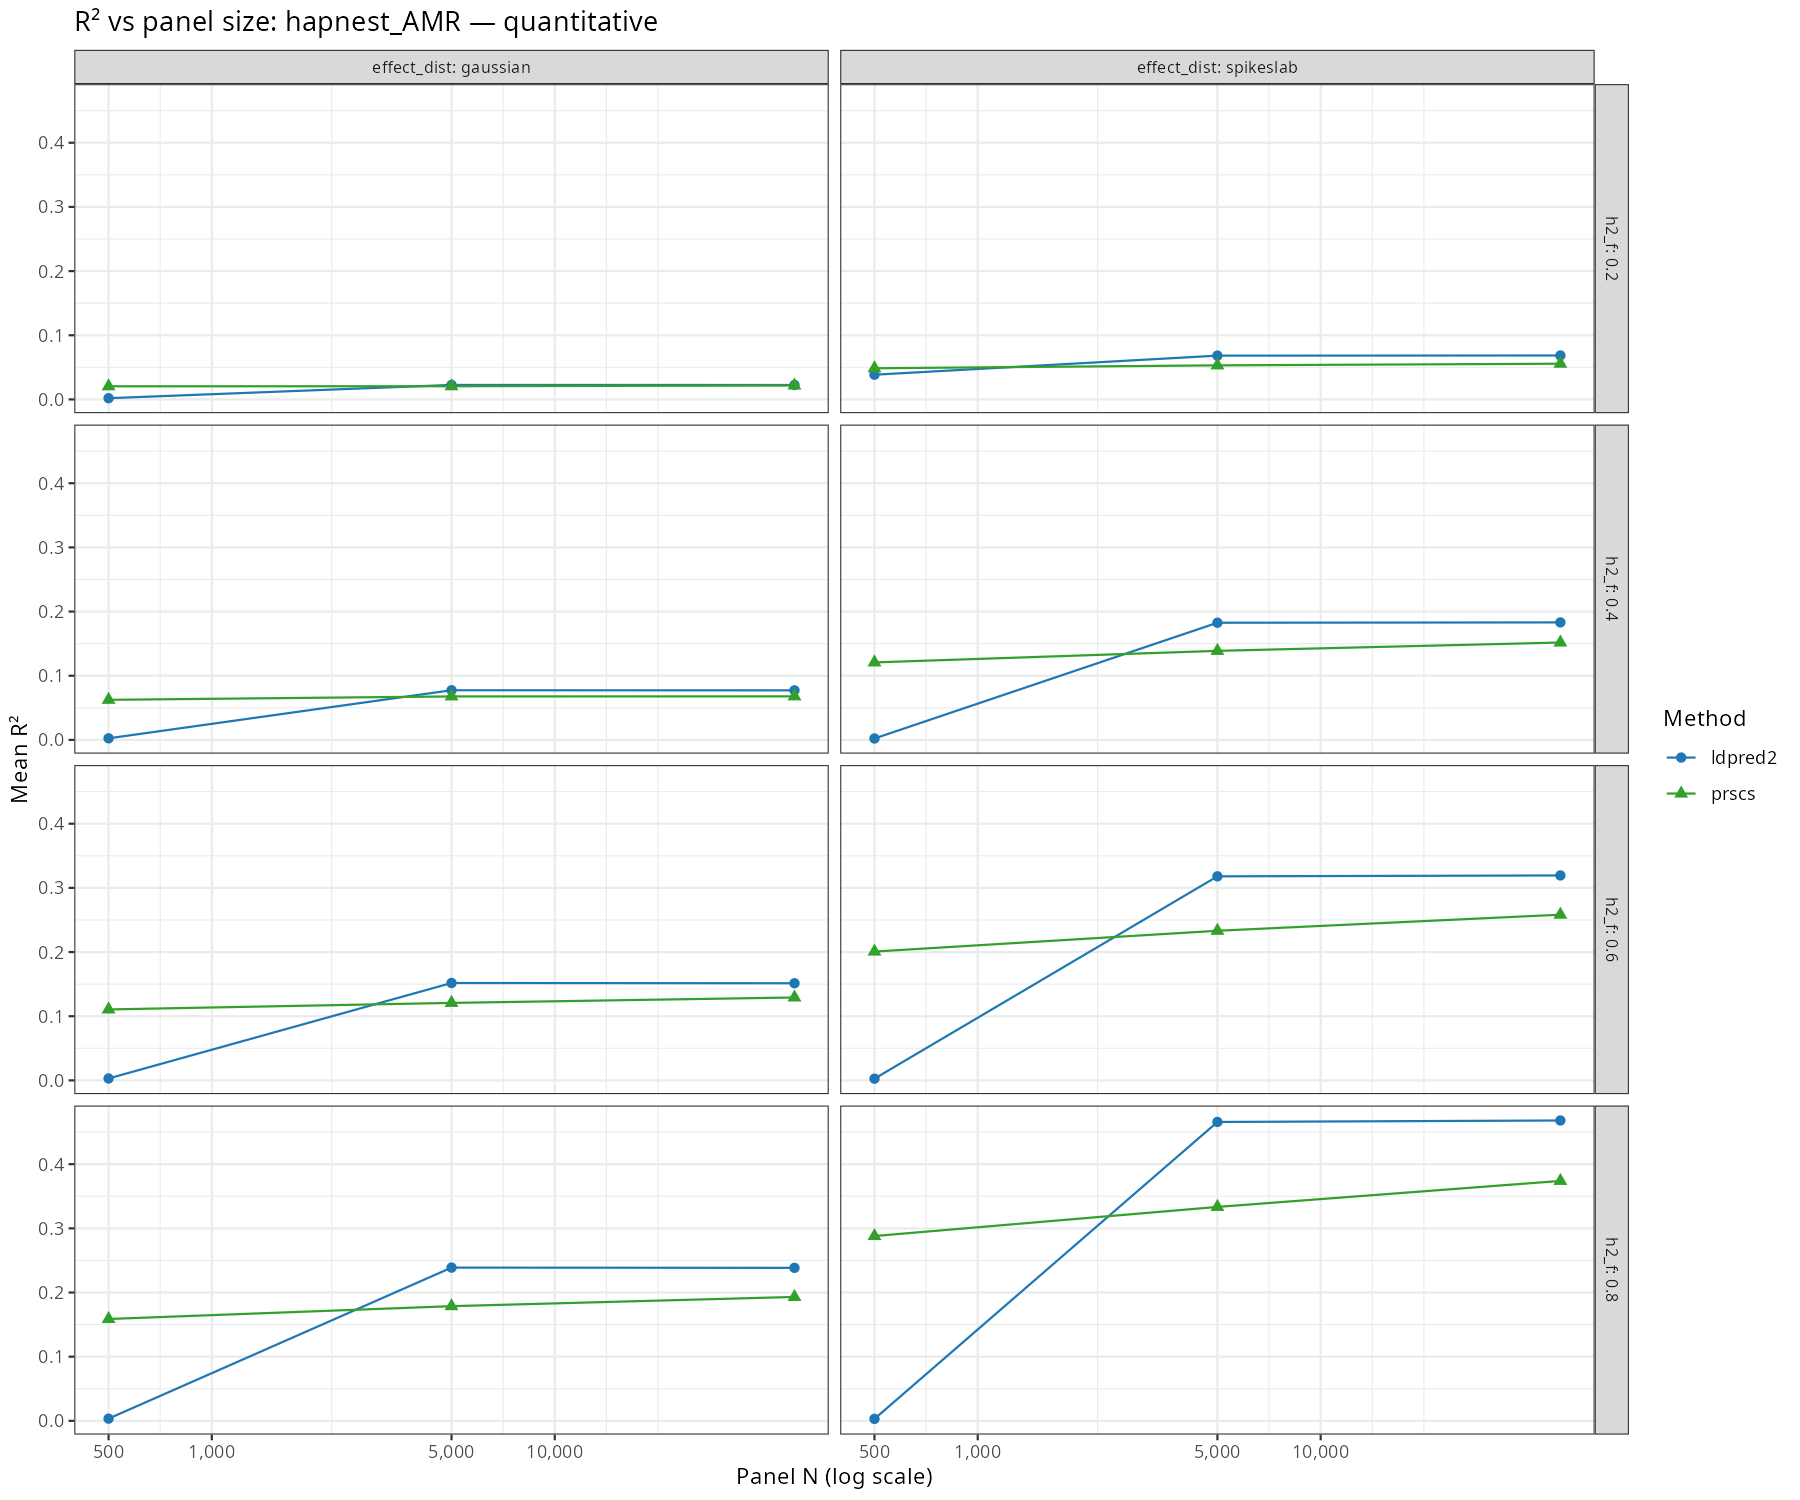
\includegraphics[width=\textwidth]{../results/summary/plots/08a_r2_amr.png}\\[0.3em]
\textbf{LDpred2} and \textbf{PRS-CS} produce similar results.
}{
%──────────── RIGHT COLUMN ─────────────────────────────────────────────────
\section{When the panel matters}
\textbf{Sparse, high-$h^{2}$ traits}
($p_{\text{causal}}\!\le\!0.01$, $h^{2}\!\ge\!0.2$):
matched-ancestry AMR panels reach $\sim$2$\times$ the $R^{2}$ of the
worst mismatched panel (EAS).
\\[0.6em]
\textbf{Panel size} drives most of its gain between
$N\!=\!500$ and $N\!=\!5{,}000$; the jump to $N\!=\!50{,}000$ adds
little.

\section{When it doesn't matter}
\textbf{Infinitesimal traits} (gaussian effects):
all six panel ancestries cluster within noise; panel size has
negligible effect.
\\[0.6em]
\textbf{Low-$h^{2}$ traits} ($h^{2}\!\le\!0.10$):
PGS accuracy is floor-limited; panel choice is a second-order concern.

\section{Implications}
For most polygenic traits the LD-panel choice is a \emph{minor}
contributor to PGS accuracy. Investment in matched-ancestry panels
pays off \textbf{primarily for sparse, high-heritability
traits}.


\section{References}
\nocite{*}
\begingroup
\renewcommand{\section}[2]{}%
\footnotesize
\bibliographystyle{unsrt}
\bibliography{references2}
\endgroup

\vspace{0.6em}
\begin{minipage}[t]{0.48\linewidth}
\centering

\includegraphics[width=0.85\linewidth]{qr_github.png}\\[0.2em]
\textbf{GitHub repository}
\end{minipage}\hfill
\begin{minipage}[t]{0.48\linewidth}
\centering

\includegraphics[width=0.85\linewidth]{qr_linkedin.png}\\[0.2em]
\textbf{LinkedIn}
\end{minipage}
}

\end{document}
